\documentclass[manuscript]{acmart}

\usepackage{graphicx}
\graphicspath{{./Source/}}

\begin{document}

    \title{A Polynomial Time Algorithm for 3SAT} 
    \author{Robert Quigley}
    % what should I do for \affiliation?
    \email{robertquigley21@gmail.com}
    % do not use \thanks for journals
    % see the acks environment sec 2.13
    % remember to put the CCS codes in!!
    
    \begin{abstract}
        This paper includes the presentation of a polynomial time algorithm to
        solve 3SAT. It begins with the problem definition and format of various
        parts of the problem. It then offers lemmas of important aspects of 
        the 3SAT problem along with their corresponding proofs. Next, it describes
        the algorithm that uses these lemmas to solve 3SAT in polynomial time. Next, it proves
        that the algorithm works for any general case of 3SAT. The algorithm relies
        on the fact that an instance of 3SAT is unsatisfiable iff contradicting
        1-terminal clauses can be derived in polynomial time. Finally it shows that, 
        because 3SAT is NP-Complete and 3SAT can be solved in polynomial time, 
        P equals NP.
    \end{abstract}
    
    % TODO: google a list of keywords for ACM journals
    \keywords{test1, test2}
    
    \maketitle 

    % \acmplain for theorem, conjecture, proposition, lemma, corollary, etc
    % \acmdefinition for example and definition
    % \acks for acknowledgements
    % bibtex or biblatex for bibliography
    
    TODO: find who the heck wrote '3SAT is NP-complete'
    read https://dl.acm.org/doi/10.1145/800157.805047

    \section{Introduction}

        This section introduces the 3SAT problem and the implications of
        solving it in polynomial time.

        As seen in (Cook's Paper),
        The boolean satisfiability problem is given as a set of terminals, $x_1, x_2, ..., x_n$,
        each of which can be assigned a value of True or False,
        combined by logical AND operators, logical OR operators, and negations.
        The problem is to determine whether or not there exists an assignment
        for each terminal that allows the instance to evaluate to True.
        As seen in (Karp's 21 NP-Complete Problems), the satisfiability problem
        with at most 3 literals per clause is NP-Complete. This is the same 
        as the boolean satisfiability problem, but it is presented such that
        a clause contains exactly three terminals combined with logical OR operators
        and possbily negation, and each clause is combined with logical AND operators.
        The idea of NP-completeness shows that if one NP-complete problem can be solved
        in polynomial time, then all problems in the class NP can be solved in polynomial time.
        In other words, P = NP.
        
    \section{Standard Definitions}

    \begin{definition}
        Terminals: symbols used in the 3SAT problem that can be assigned a value
        of either 0 or 1, True or False, or any other binary assignment. They usually
        take the form $x_i$ where $i$ is a natural number.
    \end{definition}
    \begin{definition}
        Terms: terminals in either the positive or negated form that appear in a clause.
        If a term is positive, then the value of the terminal will be the 
        same as the value of the term. If a term is negated, then the value
        of the terminal will be the opposite of the value of the term.
    \end{definition}
    \begin{definition}
        Clauses: a set of terms combined by logical OR operators.
        Clauses usually take the form 
        $(x_i \lor \neg x_j \lor x_k)$ where $x_i \neq x_j \neq x_k$
    \end{definition}
    \begin{definition}
        (3SAT) Instance: a set of any number of clauses combined by logical
        AND operators. Terminals may
        not repeat within a clause, but they are free to repeat between clauses. 
        Instances usually take the form:

        $(x_i \lor \neg x_j \lor x_k) \land (x_l \lor x_m \lor x_n)$
    \end{definition}
    \begin{definition}
        Assignment: A list of values in which each value represents either True
        or False such that each item in the list corresponds to a terminal and 
        all terminals are assigned a value.
    \end{definition}
    \begin{definition}
        Satisfying Assignment: An assignment, $A$, is said to satisfy the instance, 
        if applying $A$ will make the instance evaluate to True.
    \end{definition}
    \begin{definition}
        Satisfiable: an instance is satisfiable iff there exists a satisfying assignment.
    \end{definition}
    \begin{definition}
        Unsatisfiable: an instance is unsatisfiable iff there does not exist a satisfying assignment.
    \end{definition}

    \section{Algorithm-Specific Definitions}
    \begin{definition}
        Blocking an Assignment: An assignment, $A$, is said to be blocked if, 
        given an instance containg the clause $C$, there is no way that $A$ can 
        satisfy the instance.
    \end{definition}
    \begin{definition}
        Implication: A clause, $C$, is said to imply another clause, $D$, if all 
        assignments blocked by $D$ are also blocked by $C$ 
    \end{definition}
    \begin{definition}
        Given Clauses: clauses which were given in the original instance.
    \end{definition}
    \begin{definition}
        Implied Clauses: clauses which are implied by the clauses in the original instance.
    \end{definition}
    \begin{definition}
        k-terminal (k-t) clause: a clause is described as a k-terminal or a k-t clause
        if there are $k$ terminals in the clause.
    \end{definition}
    \begin{definition}
        Reduction: A special type of implication in which the implied 
        clause is shorter than the implying clause(s).
    \end{definition}
    \begin{definition}
        Expansion: A special type of implication in which the 
        implied clause is longer than the implying clause(s).
    \end{definition}
    \begin{definition}
        Contradicting Clauses: A set of clauses is said to be contradicting if
        they block every assignment.
    \end{definition}

    \section{Reformatting}

    Since there are a lot of constant characteristics about an instance of 3SAT, 
    we can remove most of them to allow ourselves to focus only on what changes
    from instance to instance. A list of unchanging characteristics follows:
    \begin{itemize}
        \item the symbol $x$
        \item logical AND operators
        \item logical OR operators
    \end{itemize}
    
    The only difference between instances, therefore, is the subscript of the terminal.
    
    Additionally, the following items will be changed to improve compatibility
    with Python code (cite python docs?) wherein an instance is expressed as
    a list of lists and each inner list represents a clause:
    \begin{itemize}
        \item parentheses will become square brackets
        \item negation symbols will become minus signs
        \item an instance may be surrounded with square brackets to show it is a list of lists
    \end{itemize}
   
    For example, the instance:
    
    $(\neg x_a \lor x_b \lor x_c) \land (x_a \lor x_d \lor x_e)$

    will be written as:

    $[[-a, b, c], [a, d, e]]$


    \section{Lemmas}

    \begin{lemma}
        A clause can block an assignment    
    \end{lemma}
    \begin{proof}
        Recall the definition of a clause blocking an assignment:
        An assignment is blocked if it does not allow the clause to evaluate to True.

        Since terms in a clause are combined by logical OR operators, a 
        clause cannot evalute to True iff all terms evalute to False.

        A term evaluates to False if it's either (1) negated and the terminal's
        value is True or (2) positive and the terminal's value is False

        Given a clause, we know there are three unique terminals and we can
        find assignments where all terms evalute to False.

        This would force the clause to evalute to False.

        Since the instance is composed of clauses combined by logical AND operators 
        and one clause evalutes to False, then the entire instance evalutes to False.

        Since the instance evaluates to False, the assignment cannot satisfy
        the instance.
    \end{proof}

    \begin{lemma}        
        For a given instance with $n$ terminals, there are $2^n$ possible assignments.
    \end{lemma}
    \begin{proof}
        An assignment for this instance consists of $n$ values, each with two possible
        values, True or False.

        Therefore, there are $2^n$ possible assignments.
    \end{proof}

    \begin{lemma}
        If a clause contains the same terminal in its negated and positive form, it will
        not block any assignments.
    \end{lemma}
    \begin{proof}

        Consider a clause containing the same terminal in both the positive and
        negative form.

        We know that terminal must either be True or False. Consider both cases:

        That terminal's value is True:
        The positive form of the terminal will be true and the clause will evaluate to true

        That terminal's value is False:
        The negative form of the terminal will be true and the clause will evaluate to true

        Since the clause evaluates to True in every case, there will never be an 
        assignment with which it is impossible to make this clause evalute to False.
    \end{proof}

    % \begin{lemma}
    %     For a given instance with $n$ terminals, there are $8 * {\binom{n}{3}}$
    %     possible 3-terminal clauses that block at least one instance.
    % \end{lemma}
    % \begin{proof}
    %     Recall from Lemma XXX 3.2 that a clause containing the same terminal in both
    %     the positive and negated form will always be true.

    %     Therefore, it will never block any assignments.

    %     Recall also that an instance containing the same terminal in the same
    %     form twice is not a valid 3SAT clause.

    %     Therefore we do not have to consider clauses containing the same terminal
    %     twice since we are concerned with clauses that block assignments.

    %     Given an instance with $n$ terminals, choose three of them to make a clause
        
    %     Once the terminals are selected, each terminal can have one of two values, either
    %     True or False

    %     There are $2 * 2 * 2$ possible clauses based on these terminals

    %     Since there are $8$ clauses for every selection of three terminals, there are
    %     $8 * {\binom{n}{3}}$ possible clauses
    % \end{proof}

    % \begin{lemma}
    %     Each assignment can be blocked by at most ${\binom{n}{3}}$ 3-terminal clauses
    % \end{lemma}
    % \begin{proof}
    %     Consider an assignment, A. WTS it is blocked by ${\binom{n}{3}}$ clauses.

    %     Recall from Lemma XXX 3.4 that an assignment is blocked based on values of
    %     the three terminals in the clause blocking it.

    %     Notice also that each of these values only has one possible option since
    %     assignments have a fixed value for each terminal.

    %     Recall assignments are of length $n$.

    %     We can choose three of the $n$ values in the assignments to fix and
    %     make a clause out of it in the following manner:

    %     if the value is False, the term is positive

    %     if the value is True, the term is negated

    %     This will create a clause that blocks the assignment.

    %     This allows us to have ${\binom{n}{3}}$ possible clauses that block an assignment.
        
    % \end{proof}

    \begin{lemma}
        Each clause of length $k$ blocks $2^{n-k}$ assignments
    \end{lemma}
    \begin{proof}
        In this proof, I will use $a, b, c$ instead of $x_a, x_b, x_c$ and
        I will use 0 and 1 instead of False and True

        Now, consider the general k-terminal clause, $C$, in an instance with
        $n$ terminals.

        As seen in Lemma 5.1, this blocks all assignments where all of the terms
        evaluate to False.

        Since the values for $k$ terminals are set, there are $n-k$ terminals left
        whose values could be 0 or 1.

        Since an assignment exists for every possible way to assign values to
        each terminal, we know an assignment exists for every possible way to
        assign a value for these $n-k$ terminals.

        There are two possible ways to assign values to these $n-k$ terminals
        so there are $2^{n-k}$ unique assignments blocked by $C$.
    \end{proof}

    % \begin{lemma}
    %     Adding clauses to an unsatisfiable instance will never make it satisfiable.
    %     Similarly, removing clauses from a satisfiable instance will never make it unsatisfiable.
    % \end{lemma}
    % \begin{proof}
    %     1. Recall that clauses block assignments and an instance is unsatisfiable if
    %     none of the possible assignments satisfy the instance, ie, an instnace is 
    %     unsatifiable if all of the assignments are blocked.

    %     Therefore, adding clauses to an instance in which all assignments are blocked
    %     will never be able to unblock an assignment and it will remain unsatisfiable.

    %     2. An instance is satisfiable if there exists a satisfying assignment, ie, 
    %     an instance is satisfiable if there is at least one assignment that's not blocked.

    %     Therefore, removing clauses will never be able to block that assignment and
    %     the instance will remain satisfiable.
    % \end{proof}

    \begin{lemma}
        For any clause, $C$, if we select a terminal, $t$, that's not in $C$ 
        then half of the assignments
        blocked by $C$ will assign True to $t$ and the other half will assign 
        False to $t$.
    \end{lemma}
    \begin{proof}
        We have a clause, $C$, of fixed yet arbitrary length:

        $[1, 2, 3, ...]$

        Now we select a terminal, $t$, that's not in $C$, say we call this
        terminal $t$.

        Want to show half of the assignments blocked by $C$ assign True to 
        $t$ and the other half assign False to $t$.

        We know there will be no overlap between these assignments because a single assignment
        cannot assign both the values True and False to the same terminal.

        Now we just have to show that exactly half of the assignments are blocked 
        by assigning either True or False to $t$.

        Let's say there are $k$ terms in C, then we know it blocks assignments 
        where all $k$ terms evaluate to False.

        By Lemma 5.4, this clause blocks $2^{n-k}$ assignments. 

        If we fix the value of $t$, then there are only $n-k-1$ terminals
        whose values could be 0 or 1. Since we have two choices per terminal
        and there are $n-k-1$ terminals, then there are $2^{n-k-1}$ assignments
        blocked by $C$ where the value of $t$ is fixed.

        Divide to get the ratio of the number of assignments blocked by adding 
        $t$ to the number of assignments blocked by $C$ without $t$:
        
        $2^{n-k-1}/2^{n-k}$

        = $2^{n - k - 1 - (n - k)}$

        = $2^{-1}$

        = $1/2$

        This shows that half of the assignments blocked by $C$ assign a fixed
        value to $t$.

        Since there are two possible values for $t$ and each block mutually
        exclusive halves of the assignments blocked by $C$, the lemma holds.

        For any clause, $C$, if we select a terminal, $t$, that's not
        in $C$ then half of the assignments blocked by $C$ will assign True
        to $t$ and the other half will assign False to $C$.
    \end{proof}

    \begin{lemma}
        Given a clause, $C$, and another clause, $D$, such that all of the 
        terms in $C$ also exist in $D$, then all of the assignments
        blocked by $D$ are also blocked by $C$.
    \end{lemma}
    \begin{proof}
        Given a clause, $C$, of a fixed yet arbitrary length:

        $[a, b, c, ...]$

        And another clause, $D$, containing all the terms in $C$ with possibly
        additional terms:

        $[a, b, c, ..., d, e, f, ...]$

        Want to show all the assignments blocked by $D$ are also blocked by $C$.

        We know that $C$ blocks all assignments that cause all the terms to evaluate
        to False.

        In other words, $C$ blocks all assignments where 
 
        $a = b = c = ... = False$

        Similarly, $D$ blocks all assignments where

        $a = b = c = ... = d = e = f = ... = False$

        Clearly all assignments consistent with the terminal assignments from $D$
        are also consistent with the terminal assignments from $C$.

        Therefore, every assignment blocked by $D$ is also blocked by $C$.
    \end{proof}

    \begin{lemma}
        Given the following restrictions:
        \begin{itemize}
            \item $A$ is a clause of length $k$
            \item $B$ is a clause of length $k$
            \item $A$ and $B$ share $k-1$ identical terms
            \item $A$ and $B$ share one terminal that is negated in one clause
            and positive in the other
            \item $C$ is a clause of length $k-1$ composed of the shared terms
            from $A$ and $B$
        \end{itemize}
        Then $A$ and $B$ imply $C$.

        % Two clauses of length k that share all the same terms, except for one in which
        % the same terminal is positive in one clause and negated in the other, implies
        % a clause of length k-1 which is composed of all the shared terminals.
    \end{lemma}
    \begin{proof}
        Given clauses consistent with the description:

        $A := [a, b, c, ... i]$

        $B := [a, b, c, ..., -i]$

        where $a, b, c, ...$ is shared between the clauses and $i$ is a 
        terminal not in $a, b, c, ...$

        Want to show this implies the described clause.

        Recall by Lemma 5.3 that the same terminal cannot appear both negated and
        positive within the same
        clause and still block an assignment, so $i$ cannot exist in $a, b, c...$

        Consider the clause

        $C := [1, 2, 3, ...]$

        We know by Lemma 5.5 that if we select a terminal that's not in $C$, say $t$, 
        then half of the assignments blocked by $C$ assign True to $t$ and the other
        half of the assignments blocked by $C$ assign False to $t$.

        Let this terminal $t$ that's not in $C$ be the terminal $i$ that's in $A$ and $B$.

        We know that $A$ blocks all assignments blocked by $C$ where $i$ is assigned
        the value of 0.

        We know that $B$ blocks all assignments blocked by $C$ where $i$ is assigned
        the value of 1.

        Since $A$ and $B$ both block mutually exclusive halves of $C$, we can
        say that $A$ and $B$ imply $C$.
    \end{proof}

    \begin{lemma}
        Given a clause, $C$, and a terminal, $t$, that's not in $C$, two 
        new clauses can be implied consisting of all the terms of $C$ 
        appended to either the positive form of $t$ or the negated form of $t$.
    \end{lemma}
    \begin{proof}
        Given a clause, $C$, and a terminal, $t$, that's not in $C$:

        $C := [a, b, c, ...]$

        We can compose two new clauses:

        $D := [a, b, c, ..., t]$

        $E := [a, b, c, ..., -t]$

        Since D and E both contain all the terminals from C, by Lemma 5.6 then
        D and E are implied by C.
        
    \end{proof}

    \begin{lemma}[Stronger Lemma 5.7]
        If two clauses share the same terminal, $t$, such that $t$ is 
        positive in one clause and negated in the other, then these clauses 
        imply a new clause which is composed of all the terms in both clauses 
        that do not have $t$.
    \end{lemma}
    \begin{proof}
        Consider two clauses, 

        $C := [a, b, c, ..., t]$
        
        $D := [d, e, f, ..., -t]$

        Where within a clause, the same terminal does not repeat, but between
        clauses the same terminal may repeat.

        Want to show we can imply a clause consistent with the lemma description:

        $E := [a, b, c, ..., d, e, f, ...]$

        Let's define some additional clauses:

        $E' := [a, b, c, ..., d, e, f, ..., t]$

        $E'' := [a, b, c, ..., d, e, f, ..., -t]$

        By Lemma 5.6, we know that $C$ implies $E'$, ie, all assignments blocked by
        $C$ are also blocked by $E'$.

        By Lemma 5.6, we know that $D$ implies $E''$.

        By Lemma 5.7, since $E'$ and $E''$ share all the same terms except 
        for $t$, which is positive in one clause and negated in the other, 
        we can create a new clause composed of all the shared terms in $E'$ 
        and $E''$.

        Such a clause is already defined as $E$.

        Now there are a couple extra cases to consider:
        
        \begin{itemize}
            \item There is some overlap between a, b, c, ... and d, e, f, ...
            \item There is the same terminal that's positive in a, b, c, ...
            and negated in d, e, f, ...
        \end{itemize}

        First, if the same term exists in a, b, c, ... and d, e, f, ..., then we
        can just remove one of the duplicates since one term being true implies an identical term being True

        Secondly, if the same terminal exists, but is of the opposite form in a, b, c, ... and d, e, f, ...
        then by Lemma 5.3, this clause will always be True and thus blocks no assignments so 
        $C$, $D$, and $E$ all block no assignments which makes the lemma vacuously true.
    \end{proof}

    \begin{lemma}
        Given two clauses of lengths $k$ and $m$ that share a terminal, $t$, which is 
        positive in one clause and negated in the other, you will be able
        to directly imply clauses of length $max(k, m)-1$ to $(k + m - 2)$ where
        the function $max(a, b)$ represents the parameter with the greatest value.
    \end{lemma}
    \begin{proof}
        The smallest clause that can be implied by clauses of length $k$ and $m$
        occur when all of the terms in one clause exist in the other.

        As such, the unique terms will come from the clause that's longer.

        Removing $t$, you are left with 1 less than the maximum of $k$ and $m$.

        The largest clause can be implied if there are no terms shared between
        the two clauses. In this case you subtract $1$ from the length of each
        clause to account for $t$ and since no duplicates will be removed, the 
        resulting clause's length is $2$ less than the sum of the lengths of 
        the clauses.
    \end{proof}

    \begin{lemma}
        Given four clauses of length k - 1, A, B, C, and D, and one clause of 
        length k, E, such that 
        \begin{itemize}
            \item A and B imply E
            \item C and E imply D
        \end{itemize}
        Then A, B, and C, imply D without having to process a clause of length k
    \end{lemma}
    \begin{proof}
        
        In the following figure, the first graph shows the implications as described, the second
        graph shows the implications we want to prove:
        
        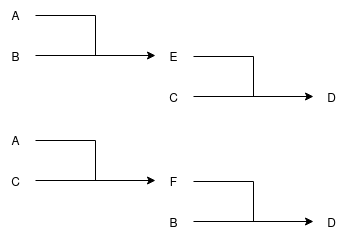
\includegraphics[scale=0.8]{317a}

        % add label to figure

        Define the clauses in the following manner:

        A := [a, b, $\beta$, i]

        B := [c, d, $\delta$ -i]

        C := [-a, e, f, $\phi$]

        Then the following are derived by Lemma 5.7:
        
        $\rightarrow$ E = [a, b, $\beta$, c, d, $\delta$]

        $\rightarrow$ D = [b, $\beta$, c, d, $\delta$, e, f, $\phi$]

        $\rightarrow$ F = [b, $\beta$, i, e, f, $\phi$]

        Where $\beta, \delta, $ and $\phi$ are sets of terms in the instance.

        Note that since $C$ and $E$ imply $D$, then $C$ and $E$ must share the
        same terminal such that it is positive in one clause and negated in the other.
        Since all of the terms in $E$ came from $A$ or $B$ (not including $i$),
        then such a term in $C$ must have the same term of the opposite form in
        $A$ or $B$ (again it cannot be $i$ since $i$ is not in $E$). And since
        $A$ and $B$ are fixed yet arbitrary sets, it does not matter which clause
        we pick as long as it is fixed for the rest of the proof. Let's pick a
        the terminal, $a$, from clause $A$.
 
        Recall from Lemma 5.3 that if a clause blocks any assignments, it cannot
        contain the same term in both forms, so if $\beta, \delta$, or $\phi$ contain
        the same terminal in both forms then $D$ blocks no assignments and the lemma 
        is vacuously true.

        We know $C$ is of length $k$ and $D$ is of length $k - 1$ or $k$.

        Consider the case where $D$ has length $k$:

        In the following equations, let the presence of a term represent a count of one,
        and the presence of a set of terms represent the number of terms in that set. If
        multiple sets of terms are shown in parentheses, let this represent the number
        of terms found in both sets.

        $k = b + c + d + e + f + \beta + \delta + \phi - (\beta \delta) - 
        (\beta \phi) - (\delta \phi) + (\beta \delta \phi)$ (by clause D)

        length of $F = b + i + e + f + \beta + \phi - (\beta \phi)$

        Want to show length of $F < k$

        $b + i + e + f + \beta + \phi - (\beta \phi) < 
        b + c + d + e + f + \beta + \delta + \phi - (\beta \delta) - 
        (\beta \phi) - (\delta \phi) + (\beta \delta \phi)$

        $\rightarrow$ $i + \beta + \phi - (\beta \phi) < 
        c + d + \beta + \delta + \phi - (\beta \delta) - 
        (\beta \phi) - (\delta \phi) + (\beta \delta \phi)$

        $\rightarrow$ $i < 
        c + d + \delta - (\beta \delta) - (\delta \phi) + (\beta \delta \phi)$

        As seen by using a Venn Diagram or other set intuition, $\delta - 
        (\beta \delta) - (\delta \phi) + (\beta \delta \phi)$, 
        represents the number of terminals in $\delta$ not in $\beta$
        and not in $\phi$.

        The lowest case for the right hand side of the inequality is where 
        this is 0, ie, all of the terms in $\delta$ are in $\beta$ or 
        $\phi$. In this case, the inequality becomes:

        $\rightarrow$ $i < c + d$

        % rephrase
        % which is guaranteed to be true since c and d both appear in B, they have to be different
        % so the length of F will always be less than k, so you do not have to process
        % clauses of length k to get the same implications.

        Which is true as long as $c$ and $d$ exist in $B$.

        WTS $c$ and $d$ always exists in $B$:

        Suppose not, then 

        $B := [\delta, -i]$

        Notice that $\delta$ is simply a fixed, yet arbitrary set of terms
        following the rules of a valid clause.

        As long as $\delta$ contains at least two terms, we can simply use 
        any two terms from $\delta$ as c and d.

        If $\delta$ does not contain two terms, then the largest possible
        length of B is 2.
        
        By Lemma 5.10, the largest clause this can imply is of length 
        $(a + b - 2)$ where $a$ is the length of $A$ and $b$ is the length 
        of $B$.

        This means the largest $E$ implied by $A$ and $B$ has the same 
        length as $A$.

        Because the lengths are equal, such a case would not allow $A$ to 
        have length $k - 1$ and $E$ to have length $k$.

        Such a case would not be consistent with the requirements of this 
        lemma and would not apply.

        Since $c$ and $d$ always exist in $B$, you can derive $D$ by processing
        clauses of length at most $k-1$.
    
        % However, you may have to process clauses up to length k - 1.

        Consider the case where the length of $D$ is $k - 1$:

        This means $k$ is one greater than the length of $D$, so $k$ is now:

        $k = b + c + d + e + f + \beta + \delta + \phi - (\beta \delta) - 
        (\beta \phi) - (\delta \phi) + (\beta \delta \phi) + 1$ (by clause D)

        Similarly as before, the inequality will become:

        $\rightarrow$ $i < c + d + 1$

        Which is again true as long as $c$ and $d$ are in $B$ and $i$ is in $A$.

        Similarly to the first half of this proof, $c$ and $d$ have to be in
        $B$.

        $i$ has to be in $A$ by the requirements of this lemma.

        Since $F$ is shorter than $E$ in all cases, the lemma holds true.
    \end{proof}

    \begin{lemma}
        Given the following:
        \begin{itemize}
            \item $A$ is a clause of length less than $k$
            \item $B$ is a clause of length $k$
            \item $C$ is a clause of length less than $k$
            \item $D$ is a clause of length $k$ or $k - 1$
            \item $A$ expands to imply $B$ by Lemma 5.6
            \item $B$ and $C$ imply $D$ by Lemma 5.9
        \end{itemize}
        Then $A$ and $C$ can imply $D$ by processing clauses of at 
        most length $k - 1$.
    \end{lemma}
    \begin{proof}

        Consider the following case:

        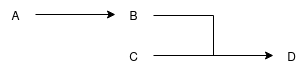
\includegraphics[scale=0.8]{318}

        A := [a, b, $\beta$]
        
        A' := [a, b, $\beta$, c]

        B := [a, b, $\beta$, c, d, $\delta$]

        $C_1$ := [-a, e, f, $\phi$]

        $C_2$ := [-c, e, f, $\phi$]

        $D_1$ := [b, $\beta$, c, d, $\delta$, e, f, $\phi$]

        $D_2$ := [a, b, $\beta$, d, $\delta$, e, f, $\phi$]

        E := [b, $\beta$, e, f, $\phi$]

        F := [a, b, $\beta$, e, f, $\phi$]

        Where $\beta, \delta$, and $\phi$ are fixed, yet arbitrary sets of terms 
        abiding by the rules for a valid clause (see Lemma 5.3) and consistent
        with the requirements of this lemma.

        Notice that $C$ has to contain a term from $B$ in the opposite form by 
        lemma 5.9.

        Notice that $B$ is made up of terms from $A$ and terms not in $A$
        by lemma 5.6.

        The term in $C$ which is opposite from the term in $B$ can therefore
        be opposite from a term
        in $A$ (in this case, use $C_1$ and $D_1$) or a 
        term not in $A$ (in this case use $C_2$ and $D_2$).
        
        Consider the opposite form term in $C$ is in $A$, ie, use $C_1$
        and $D_1$:

        Notice $A$ and $C_1$ share an opposite term, then they can derive
        a clause, $E$, by Lemma 5.9:

        And $E$ can imply a clause $D_1$ by Lemma 5.6:

        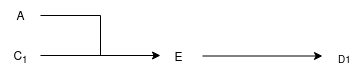
\includegraphics[scale=0.8]{318b.png}

        % label the graphic

        Want to show you only have to process clauses whose length is
        less than $k$ to derive $D_1$.

        Want to show length of $E$ is less than $k$.

        Consider two cases: (1) $D$ is of length $k$ and 
        (2) $D$ is of length $k - 1$
        
        Consider (1) where $D$ is of length $k$:

        Since $D$ is of length $k$, we can define $k$ as follows:

        $k = b + c + d + e + f + \beta + \delta + \phi - (\beta \delta) 
        - (\beta \phi) - (\delta \phi) + (\beta \delta \phi)$

        Length of $E = b + e + f + \beta + \phi - (\beta \phi)$
        
        WTS length of $E is less than k$:

        $b + e + f + \beta + \phi - (\beta \phi) < b + c + d + e + f + 
        \beta + \delta + \phi - (\beta \delta) - (\beta \phi) - (\delta \phi) 
        + (\beta \delta \phi)$

        $\rightarrow 0 < c + d + \delta - (\beta \delta) 
        - (\delta \phi) + (\beta \delta \phi)$

        Using a Venn Diagram or by other set intuition, $\delta - 
        (\beta \delta) - (\delta \phi) + (\beta \delta \phi)$ represents
        the number of terms in $\delta$ not in $\beta$ and not in $\phi$. 
        The lowest this value can be is 0 if all terms in $\delta$ are in 
        $\beta$ or $\phi$.

        The inequality becomes:

        $\rightarrow 0 < c + d$

        Which is true as long as $c$ or $d$ exist in $B$.

        WTS $c$ or $d$ always exists in $B$.

        Suppose not, then:

        $B := [a, b, \beta]$

        Note that the maximum length of $\delta$ is 0 because if it were 1
        or more, then we can just extract $c$ or $d$ from $\delta$.

        In this case, the length of $B$ is the same as the length of $A$ and 
        it is impossible for the lemma requirements defining the lengths
        of $A$ and $B$ to hold.

        Therefore, $c$ or $d$ must always exist in $B$.

        Since $c$ or $d$ must exist in $B$, the inequality is always true, 
        and the length of $E$ is indeed less than $k$.

        Consider (2) $D$ is of length $k - 1$:

        Then the length of $k$ is redefined as:

        $k = b + c + d + e + f + \beta + \delta + \phi - (\beta \delta) 
        - (\beta \phi) - (\delta \phi) + (\beta \delta \phi) + 1$

        Similarly as before, the inequality becomes:

        $\rightarrow 0 < c + d + 1$

        Which is always true so the length of $E$ is indeed less than $k$.

        Notice that, by lemma 5.6, you only have to process clauses of length
        at most $k-1$ to derive a clause of length $k$, in context, you 
        can derive $D$ via expansion while only processing clauses with
        a maximum length of $k-1$.

        % rephrase
        % Since expanding a clause only directly implies clauses of length 1 greater, 
        % you only have to process clauses of at most length k - 1 to derive D

        Consider the case using $C_2$ and $D_2$:

        We can construct a clause, $A'$, such that $A$ expands to $A'$ by 
        lemma 5.6 and there is a term in $A'$ whose opposite term is in $C_2$.

        By lemma 5.9, $A'$ and $C_2$ imply a clause, $F$.

        And by lemma 5.6, all the terms in $F$ are in $D_2$ so $F$ implies $D_2$.

        This is seen in the following graphic:

        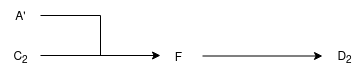
\includegraphics[scale=0.8]{318c.png}
        
        Want to show $A'$ and $F$ are shorter than $k$.

        First, Want to show the length of $A'$ is less than $k$:

        Consider two cases, (1) $D_2$ is of length $k$ and 
        (2) $D_2$ is of length k - 1

        Consider (1) $D_2$ is of length $k$, then we can define k as follows:

        $k = b + c + d + e + f + \beta + \delta + \phi - (\beta \delta) 
        - (\beta \phi) - (\delta \phi) + (\beta \delta \phi)$

        length of $A' = a + b + \beta + c$

        Want to show the length of $A'$ is less than $k$:

        $\rightarrow$ $a + b + \beta + c$ $<$ $b + c + d + e + f + 
        \beta + \delta + \phi - (\beta \delta) 
        - (\beta \phi) - (\delta \phi) + (\beta \delta \phi)$

        $\rightarrow$ $a$ $<$ $d + e + f + \delta + \phi - (\beta \delta) 
        - (\beta \phi) - (\delta \phi) + (\beta \delta \phi)$

        By Venn Diagram or other set intuition, 
        $\delta + \phi - (\beta \delta) - (\beta \phi) - (\delta \phi) + 
        (\beta \delta \phi)$ represents the number of unique terms in 
        $\delta$ and $\phi$
        The smallest value for this is when $\delta = \phi$, so this can
        be replaced with $\phi$.

        $\rightarrow$ $a$ $<$ $d + e + f + \phi$

        Which is true as long as there are at least two terms in $d, e, f, \delta$ or $\phi$

        Want to show at least two terms have to exist in d, e, f, $\delta$, or $\phi$.

        Suppose not, then the largest $D_2$ is

        $D_2 := [a, b, \beta, x]$

        Where $x$ is a single term from $\{d, e, f, \delta, \phi\}$

        The clause $A$ can clearly expand to $D_2$ by Lemma 5.6. 
        
        Since $D_2$ is of length $k$, it can be expanded to by processing
        only clauses with a maximum length of $k-1$.

        Therefore any case where there are fewer than two terms in 
        $\{d, e, f, \delta, \phi\}$, will allow the lemma to hold.

        Consider (2) $D_2$ is of length $k - 1$:

        $k$ is now defined as:

        $k = b + c + d + e + f + \beta + \delta + \phi - (\beta \delta) 
        - (\beta \phi) - (\delta \phi) + (\beta \delta \phi) + 1$

        Similarly as before, the inequality becomes:

        $\rightarrow$ $a$ $<$ $d + e + f + \delta + 1$

        Which is true as long as there is at least one term in
        $d, e, f, \delta$ or $\phi$.

        As seen before, if there are fewer than two terms in
        $\{d, e, f, \delta, \phi\}$ then the lemma already holds.

        Therefore if $D_2$ is of length $k - 1$, the length of $A'$ is 
        shorter than $k$.
        
        Secondly, want to show $F$ is shorter than $k$.

        Consider two cases, (1) $D_2$ is of length $k$ and 
        (2) $D_2$ is of length $k - 1$.

        Consider (1) where $D_2$ is of length $k$:
        
        By $D_2$, $k$ is defined as 

        $k = b + c + d + e + f + \beta + \delta + \phi - (\beta \delta) 
        - (\beta \phi) - (\delta \phi) + (\beta \delta \phi)$

        length of $F = a + b + e + f + \beta + \phi - (\beta \phi)$
        
        WTS length of $F$ is less than $k$:

        $a + b + e + f + \beta + \phi - (\beta \phi)$ $<$ 
        $b + c + d + e + f + \beta + \delta + \phi - (\beta \delta) 
        - (\beta \phi) - (\delta \phi) + (\beta \delta \phi)$

        $\rightarrow$ $a$ $<$ $c + d + \delta - (\beta \delta) - 
        (\delta \phi) + (\beta \delta \phi)$

        Using a Venn Diagram or by other set intuition, 
        $\delta - (\beta \delta) - (\delta \phi) + (\beta \delta \phi)$
        represents the terms in $\delta$ that are not in $\beta$ or $\phi$.
        
        This is lowest when all the terms in $\delta$ are in $\beta$ or $\phi$, 
        this part of the inequality then becomes 0.

        Then the inequality becomes:

        $\rightarrow$ $a$ $<$ $c + d$

        Which is true if $c$ and $d$ exist.

        WTS $c$ and $d$ exist.

        Suppose not, then

        $B := [a, b, \beta, x]$

        where $x$ is a single term. Note that if $x$ is more than one term,
        then we could use the two terms in $x$ as $c$ and $d$.

        Here we can use $x$ as $c$ and $B$ becomes equivalent to $A'$, 
        which was already shown to be shorter than $k$.

        Consider (2) where $D_2$ is of length $k - 1$.

        Then $k$ is defined as:

        $k = b + c + d + e + f + \beta + \delta + \phi - (\beta \delta) 
        - (\beta \phi) - (\delta \phi) + (\beta \delta \phi) + 1$

        Want to show length of $F$ is less than $k$:

        $a + b + e + f + \beta + \phi - (\beta \phi)$ $<$ 
        $b + c + d + e + f + \beta + \delta + \phi - (\beta \delta) 
        - (\beta \phi) - (\delta \phi) + (\beta \delta \phi) + 1$

        Similarly as before, this becomes:

        $\rightarrow$ $a$ $<$ $c + d + 1$

        Which is always true since we already proved $c$ and $d$ have to exist.

        Since $F$ is smaller than $k$ and $D_2$ has a maximum length of $k$, 
        and by Lemma 3.6 the largest a clause has to be in order to imply
        another clause of length $k$ is $k-1$. Meaning you only have to process
        clauses of length $k-1$ in order to derive a clause of length $k$.
        
        Since $A, C_1, C_2, E, and F$ are all shorter than $k$ and $D$ can
        be derived by expanding $E$ or $F$, then $D$ can be derived from $A$
        and $C$ without the need to process clauses of length greater than $k - 1$.
    \end{proof}

    % \begin{lemma}
    %     Using Lemma 5.10, a 1-t clause can only be directly implied by two 2-t clauses sharing
    %     the same terminal with the other terminal positive in one clause and 
    %     negated in the other.
    % \end{lemma}
    % \begin{proof}
    %     Given a 1-t clause, 
        
    %     [i]

    %     WTS that it can only be directly implied by 2-t clauses like 

    %     [i, j]

    %     [i, -j]

    %     By Lemma XXX 3.13, the smallest clause that can be derived from two
    %     clauses of length k and l is max(k, l) - 1.

    %     With k = l = 2, this gives us a clause of length 1.

    %     If we increase by the lowest possible amount, say k = 3, l = 2, this
    %     gives us a clause of length 2.

    %     So we have to use two clauses of length 2 if we want to directly imply
    %     a clause of length 1 by using the algorithm.

    %     By the algorithm, both clauses must share the same terminal, where it's 
    %     positive in one clause and negative in the other.

    %     Now each clause has one remaining terminal and they could either be (1)
    %     the same terminal or (2) different terminals.

    %     \begin{enumerate}
    %         \item The same term:
            
    %         By Lemma XXX 3.12 or more directly Lemma XXX 3.10, this will derive a 1-t clause
            
    %         \item Different term:
            
    %         By Lemma XXX 3.12, this will derive a 2-t clause
    %     \end{enumerate}

    %     Therefore, using Lemma XXX 3.12, a 1-t clause can only be directly implied by 
    %     two 2-t clauses sharing the same terminal with the other terminal positive
    %     in one clause and negated in the other.

    % \end{proof}

    \begin{lemma}
        Given an instance of 3SAT, you can expand all of the given clauses
        to the point where you are considering clauses of length $n$.
    \end{lemma}
    \begin{proof}
        Given an instance of 3SAT, we know all clauses are of length 3.

        If we want to consider a generic $n$-terminal, $B$, that's implied by a
        given clause, $A$, then by Lemma 5.6 we know it's implied iff it $B$ 
        contains all of the terms in $A$.
    \end{proof}

    \begin{lemma}
        If you expand given 3-t clauses as described in Lemma 5.13, you will
        derive $2^n$ unique clauses of length $n$ iff the instance is unsatisfiable.
    \end{lemma}
    \begin{proof}
        Want to show an unsatifiable instance implies $2^n$ unique n-terminal
        clauses can be derived from the given 3-t clauses:

        By lemma 5.4, a clause of length $n$ blocks 1 assignment. 

        Recall an instance is unsatisfiable iff all $2^n$ assignments are
        blocked.

        If a 3-terminal clause blocks an assignment, then it also implies
        the corresponding n-terminal assignment because there is one possible
        n-terminal clause for any assignment.

        Since all assignments are blocked, there exists a 3-terminal clause for each
        assignment such that the terminals in the clause are assigned to make
        the clause evalute to false.

        Similarly, for each assignment, there exists an n-terminal clause such
        that the terminals in the clause are assigned to make the clause evaluate
        to false.

        This will create a unique n-terminal clause for each assignment since
        each clause can block only one assignment and overlap would imply
        the same terminal having two values in the same assignment.

        Notice that for each of these n-terminal clauses, they must contain
        three terms from at least one given clause. If they didn't, then
        the assignment blocked by that n-terminal clause would not be blocked
        and the instance would be satisfiable.

        WTS if $2^n$ unique n-terminal clauses are derived by the given
        3-t clauses, then the instance is unsatifiable.

        By lemma 5.4, a clause of length $n$ blocks 1 assignment. 

        Therefore if there are $2^n$ unique n-terminal clauses, then
        all $2^n$ assignments will be blocked.

        Note that there will be no overlap because each n-terminal clause
        sets the value for each terminal and overlap would imply a terminal
        having two values at the same time.
    \end{proof}

    \begin{lemma}
        The n-terminal clauses described in Lemma 5.14 can be reduced to derive
        any pair of contradicting 1-terminal clauses.
    \end{lemma}
    \begin{proof}
        Given $2^n$ n-terminal clauses, want to show you can imply any pair
        of contradicting 1-terminal clauses by lemma 5.7.

        Pick a terminal that will not exist in the final 1-terminal clauses.

        Half of the existing n-terminal clauses have that terminal assigned
        the value of False and the other half have that terminal assigned
        the value of True.

        Pick one clause that blocks an assignment where the terminal is True.

        Then there exists an assignment/n-terminal clause for each possible
        value for the remaining n-1 terminals.

        Therefore, there must exist another clause that shares all of the same terms, but
        where that one terminal is assigned the value of False.

        Using these two terms, we can create a new clause by lemma 5.7.

        Now all of the clauses of length n - 1 do not contain that terminal.

        Forget that terminal is part of the problem and repeat this process
        until you are left with two contradicting 1-terminal clauses.
    \end{proof}

    \begin{lemma}
        Contradicting 1-terminal clauses can be expanded to imply
        every possible 3-terminal clause.
    \end{lemma}
    \begin{proof}
        Let the following clauses be a pair of contradicting 1-t clauses:

        [a]

        [-a]

        By lemma 5.6, we can expand to any clause that contains $a$ or $-a$.

        Let the following be a generic 3-terminal clause that does not contain
        $a$ or $-a$:

        [b, c, d]

        By Lemma 5.6, we know the 1-terminal clauses imply the following 3-t clauses:

        [a, b, c]

        [-a, b, d]

        By Lemma 5.9, these clauses imply:

        [b, c, d]
    \end{proof}

    % \begin{lemma}
    %     Any unsatifiable instance can be converted to a form such that if one 3-terminal
    %     clause is removed, the instance will be satisfiable.
    % \end{lemma}
    % \begin{proof}
    %     TODO Prove    
    % \end{proof}


    \section{Algorithm}

    \begin{enumerate}
        \item For each clause in the instance, C, of length 3 or less:
        \begin{enumerate}
            \item For each clause in the instance, D, of length 3 or less:
            \begin{enumerate}
                \item Get all clauses implied by C and D according to Lemma 5.9 
                and add them to the instance
            \end{enumerate}
            \item For each clause in the instance, E, of length 1:
            \begin{enumerate}
                \item For each clause in the instance, F, of length 1:
                \begin{enumerate}
                    \item if E and F contain the same terminal in which it is 
                    positive in one clause and negated in the other, the 
                    clauses are contradicting and the instance is unsatisfiable, end
                \end{enumerate}
            \end{enumerate}
        \end{enumerate}
        \item Repeat (1) until no new clauses are added
        \item If it reaches here, the instance is satisfiable, end
    \end{enumerate}

    \section{Time Complexity Analysis}

    In this section I will analyze the time complexity of the algorithm in section 4

    (1) At most ${\binom{n}{3}}*8 + {\binom{n}{2}}*4 + {\binom{n}{1}}*2$ clauses to iterate which is on the order of

    $O(n^3)$

    (1.a) At most ${\binom{n}{3}}*8 + {\binom{n}{2}}*4 + {\binom{n}{1}}*2$ clauses to iterate which is on the order of

    $O(n^3)$

    (1.a.i) For each terminal in C, check if it's opposite form is in D

    $O(3^2)$ which is just constant time which is on the order of 

    $O(1)$

    (1.b) At most ${\binom{n}{1}} * 2$ clauses of length 1 exist, which is on the order of

    $O(n)$

    (1.b.i) At most ${\binom{n}{1}} * 2$ clauses of length 1 exist, which is on the order of

    $O(n)$

    (1.b.i.A) Constant time to check if two 1-terminal clauses contain the same terminal in the opposite form

    $O(1)$

    (2) Worst case, we add one new clause each time so we have to do (1) ${\binom{n}{3}} * 8 + {\binom{n}{2}} * 8 + {\binom{n}{1}} * 2$ which is on the order of

    $O(n^3)$

    (3) Constant time to check and return satisfiable

    $O(1)$

    The time complexity breaks down:

    $(2) * ((1) * ((1.a) * ((1.a.i)) + (1.b) * ((1.b.i) * (1.b.i.A)))) + (3)$

    $= O(n^3) * (O(n^3) * (O(n^3) * (O(1)) + O(n) * (O(n) * O(1)))) + O(1)$

    $= O(n^3) * (O(n^3) * (O(n^3) * (O(1)) + O(n) * O(n))) + O(1)$

    $= O(n^3) * (O(n^3) * (O(n^3) * (O(1)) + O(n^2))) + O(1)$

    $= O(n^3) * (O(n^3) * (O(n^3) + O(n^2))) + O(1)$

    $= O(n^3) * (O(n^3) * O(n^3)) + O(1)$

    $= O(n^3) * O(n^6) + O(1)$

    $= O(n^9) + O(1)$

    $= O(n^9)$

    \section{Proof of Correctness}

    By Lemma 5.12, if we expand to a clause, $B$, of length $k$, then
    use $B$ and another clause, $C$, of length less than $k$, to imply
    a new clause, $D$, of length at most $k$ by lemma 5.9, then
    we can derive $D$ by processing clauses of at most length $k-1$.



    ---

    By Lemma XXX 3.18/Lemma XXX 3.17, if we can derive a clause of length k, say C, then
    any clause of length k - 1, say D, can be implied by 
    the clauses implying C without the need to process a clause of length 
    k or greater.

    Now, WTS an unsatisfiable instance means we will imply contradicting 1-t clauses.

    Given an unsatisfiable instance, we can expand the 3-t clauses to produce
    all possible n-terminal clauses.

    These n-terminal clauses imply clauses of length n or n-1 using the algo.

    They cannot imply any new n-terminal clauses since we already have all possible
    n-terminal clauses since it's unsatisfiable.

    And by Lemma XXX 3.18, the n-1-terminal clauses that are implied can be implied
    without having to process clauses longer than n - 1.

    Now we have all the n-1-terminal clauses. These imply clauses between
    lengths n-2 and 2(n-1) - 2 by Lemma XXX 3.13.

    We already have the clauses longer than n-1 so we really only care about
    implying the clauses of length n-2. 

    Again by Lemma XXX 3.18, these clauses can be implied without having to
    process clauses greater than length n-2.

    Continue this pattern...

    We already have the clauses of length n-w and we already derived any clause
    longer than n-w so the only clauses left are the clauses of length n-w-1.
    By Lemma XXX 3.18/Lemma XXX 3.17, we can derive the clauses of length n-w-1 without
    processing clauses longer than n-w-1.

    Continue ...

    We already have clauses of length 4 and we already derived any clause greater
    than length 4 so the only clauses left to imply are those of length 3.
    By Lemma XXX 3.18/Lemma XXX 3.17, we can derive the clauses of length 3 without processing
    clauses greater than length 3. 

    Now we have all the clauses of length 3, and clearly a path exists to derive
    contradicting 1-terminal clauses.

    And since we do not have to process clauses of length greater than 3, the 
    time complexity analysis in section 5 holds and it is indeed polynomial time.

    But wait! What if we get the retort: 
    Consider "we already have all clauses of length 3, doesn't Lemma XXX 3.17/ Lemma XXX 18 mean
    any 2-terminal clause implied by these can already be implied without 
    processing a clause of length 3?"
    No, because the given 3-terminal clauses were not derived, so some processing
    does have to happen.


    \section{Conclusion} 

    In this paper, we present an algorithm to solve 3SAT in polynomial time.

    By the (Karp's paper), 3SAT is NP-complete, meaning 3SAT is at least
    as hard as every problem in NP.
    
    Since we have an algorithm to solve 3SAT in polynomial time, then all problems
    in NP can be solved in polynomial time.

    Thus, P = NP. 

    % example citation
    % \cite{knuth:1984}
    % \bibliography{refs}
    % \bibliographystyle{plain}

    TODO:
    \begin{itemize}
        \item reorder definitions
        \item redo Lemma 3.18
        \item Perhaps modify the algo to use expansion or add another lemma
        to say 'expansion is equivalent to the current algo if we only deal with
        1-, 2-, 3-, terminal clauses'
    \end{itemize}


\end{document} 